\documentclass[11pt,a4paper]{article}

% ── Packages ──────────────────────────────────────────────────────────────────
\usepackage[margin=2.5cm]{geometry}
\usepackage{amsmath,amssymb}
\usepackage{booktabs}
\usepackage{multirow}
\usepackage{array}
\usepackage{pgfplots}
\pgfplotsset{compat=1.18}
\usepackage{pgfplotstable}
\usepackage{hyperref}
\usepackage{caption}
\usepackage{subcaption}
\usepackage{authblk}
\usepackage{microtype}
\usepackage{siunitx}
\sisetup{round-mode=places, round-precision=2}

% ── Meta ──────────────────────────────────────────────────────────────────────
\title{\textbf{Experimental Analysis of Strip Packing Algorithms}\\[0.4em]
       \large Comparative Study of Exact, Constructive, and Shelf Heuristics\\
       with Machine Learning Algorithm Selection}
\author{[Your Name]}
\affil{[Your Department / University]}
\date{May 2026}

\begin{document}
\maketitle
\tableofcontents
\bigskip

% ── Abstract ──────────────────────────────────────────────────────────────────
\begin{abstract}
We present an experimental analysis of five algorithms for the
Two-Dimensional Strip Packing Problem (2SP): the Bottom-Left-Fill (BLF)
constructive heuristic with four sorting strategies, the Next Fit Decreasing
Height (NFDH) shelf heuristic, the First Fit Decreasing Height (FFDH)
shelf heuristic, and an exact method based on Google OR-Tools CP-SAT
constraint programming.
Experiments are conducted on 60 benchmark instances drawn from the
Bengtsson (1982), Berkey \& Wang (1987), and Martello \& Vigo (1998) families.
We additionally train a Random Forest classifier on 17 geometric instance
features to automatically select the best-performing heuristic for an
unseen instance.
Results show that BLF (best-of-four) achieves an average gap of
\(\approx7\%\) above the area lower bound, while shelf methods are
faster but generally produce larger gaps.
The ML selector matches or improves upon the manually chosen strategy
in cross-validation.
\end{abstract}

% ──────────────────────────────────────────────────────────────────────────────
\section{Introduction}
% ──────────────────────────────────────────────────────────────────────────────

The \emph{Two-Dimensional Strip Packing Problem} (2SP) asks: given a strip of
fixed width \(W\) and an unbounded height, and a set of \(n\)
axis-aligned rectangles \(\{(w_i, h_i)\}_{i=1}^{n}\), pack all rectangles
into the strip without overlap and minimise the resulting height \(H\).
The problem is NP-hard in the strong sense \cite{GareyJohnson1979}.

Practical applications include paper and sheet metal cutting, VLSI floorplanning,
advertisement placement, and container loading.
This report evaluates the algorithms listed in Table~\ref{tab:algorithms}.

\begin{table}[h]
\centering
\caption{Algorithms studied in this report.}
\label{tab:algorithms}
\begin{tabular}{llll}
\toprule
\textbf{ID} & \textbf{Algorithm} & \textbf{Class} & \textbf{Complexity} \\
\midrule
BLF-DH & BLF, Decreasing Height & Constructive heuristic & $O(n^3)$ \\
BLF-DW & BLF, Decreasing Width  & Constructive heuristic & $O(n^3)$ \\
BLF-DA & BLF, Decreasing Area   & Constructive heuristic & $O(n^3)$ \\
BLF-DP & BLF, Decreasing Perimeter & Constructive heuristic & $O(n^3)$ \\
NFDH   & Next Fit Decreasing Height & Shelf heuristic      & $O(n\log n)$ \\
FFDH   & First Fit Decreasing Height & Shelf heuristic     & $O(n^2)$ \\
CP-SAT & OR-Tools CP-SAT        & Exact (60\,s limit)   & Exponential \\
ML     & Random Forest Selector & Algorithm selection   & $O(1)$ inference \\
\bottomrule
\end{tabular}
\end{table}

% ──────────────────────────────────────────────────────────────────────────────
\section{Problem Formulation}
% ──────────────────────────────────────────────────────────────────────────────

Let \(\mathcal{R} = \{(w_i, h_i)\}_{i=1}^n\) be the set of rectangles and
\(W \in \mathbb{Z}^+\) the strip width.
The placement of rectangle \(i\) is determined by its bottom-left corner
\((x_i, y_i)\).
The optimisation problem is:
\begin{align}
\text{minimise} \quad & H \label{eq:obj}\\
\text{subject to} \quad
  & x_i + w_i \le W, \quad y_i + h_i \le H, \quad x_i,y_i \ge 0
    \quad \forall i \label{eq:bounds}\\
  & \text{no overlap between any two rectangles.} \label{eq:nooverlap}
\end{align}

A useful lower bound is the \emph{area lower bound}:
\begin{equation}
\mathrm{LB}_{\text{area}} = \left\lceil \frac{\sum_{i=1}^n w_i h_i}{W} \right\rceil.
\label{eq:lb}
\end{equation}
The \emph{gap} of a solution with height \(H\) relative to this bound is:
\begin{equation}
\mathrm{Gap} = \frac{H - \mathrm{LB}_{\text{area}}}{\mathrm{LB}_{\text{area}}} \times 100\%.
\label{eq:gap}
\end{equation}

% ──────────────────────────────────────────────────────────────────────────────
\section{Algorithms}
% ──────────────────────────────────────────────────────────────────────────────

\subsection{Bottom-Left-Fill (BLF)}

BLF is a greedy constructive heuristic introduced by Baker et al.~\cite{Baker1980}
and formalised by Chazelle~\cite{Chazelle1983}.
After sorting the rectangles by a chosen key, each rectangle is placed at
the \emph{lowest} feasible $y$-coordinate, then as far \emph{left} as
possible at that level.
Candidate $y$-levels are $\{0\} \cup \{y_j + h_j : j \text{ placed}\}$, i.e.\
the bottom of the strip or the top edge of any placed rectangle.
Similarly, candidate $x$-positions are $\{0\} \cup \{x_j + w_j\}$.

Four item orderings are compared:
\textbf{DH} (decreasing height), \textbf{DW} (decreasing width),
\textbf{DA} (decreasing area), and \textbf{DP} (decreasing perimeter).

\subsection{Shelf Heuristics (NFDH, FFDH)}

Shelf heuristics \cite{Coffman1980} pack items in horizontal \emph{shelves}.
Items are sorted by decreasing height.

\textbf{NFDH}: keeps one open shelf; when the next item does not fit horizontally,
closes the shelf and starts a new one.
Approximation ratio: $H \le 2 \cdot \mathrm{OPT} + h_{\max}$.

\textbf{FFDH}: for each item scans all open shelves from the bottom and
places it on the \emph{first} shelf where it fits; opens a new shelf only if
none suffices.
Approximation ratio: $H \le \tfrac{17}{10} \cdot \mathrm{OPT} + h_{\max}$.

\subsection{Exact Solver (CP-SAT)}

The exact formulation uses Google OR-Tools CP-SAT \cite{ORTools}.
Each rectangle is modelled with a pair of fixed-size interval variables
$(x_i, x_i + w_i)$ and $(y_i, y_i + h_i)$, and the \texttt{AddNoOverlap2D}
global constraint enforces non-overlap efficiently via propagation.
The objective minimises the auxiliary variable $H \ge y_i + h_i$ for all $i$.
A wall-clock time limit of 60 seconds is applied; the solver returns
\textsc{Optimal}, \textsc{Feasible}, or \textsc{Unknown}.

\subsection{ML Algorithm Selector}

We extract 17 dimensionless features from each instance
(see Table~\ref{tab:features}) and train a Random Forest classifier
(\texttt{n\_estimators}=300, \texttt{max\_features}="sqrt") to predict
which of the six heuristics will yield the smallest height.
Training labels are obtained by running all six heuristics on all 60
benchmark instances and recording the winner.
Inference is $O(1)$ and adds negligible overhead to the selected heuristic.

\begin{table}[h]
\centering
\caption{Instance features used by the ML selector.}
\label{tab:features}
\small
\begin{tabular}{lll}
\toprule
\# & Feature & Description \\
\midrule
1  & $n$          & Number of rectangles \\
2  & $W$          & Strip width \\
3  & $\mathrm{LB}_{\text{area}}$ & Area lower bound \\
4--7 & $\bar{w}/W$, $\sigma_w/W$, $\max w/W$, $\min w/W$ & Width statistics (norm.\ by $W$) \\
8--11 & $\bar{h}/\mathrm{LB}$, $\sigma_h/\mathrm{LB}$, $\max h/\mathrm{LB}$, $\min h/\mathrm{LB}$ & Height statistics (norm.\ by LB) \\
12--13 & $\overline{w/h}$, $\sigma_{w/h}$ & Aspect-ratio mean and std \\
14 & $\overline{w_ih_i}/(\mathrm{LB}\cdot W)$ & Mean item area / strip area \\
15 & $\sum w_ih_i / (\mathrm{LB}\cdot W)$ & Packing density at LB height \\
16 & fraction of items with $w_i > W/2$ & Wide-item fraction \\
17 & fraction of items with $h_i > \bar{h}$ & Tall-item fraction \\
\bottomrule
\end{tabular}
\end{table}

% ──────────────────────────────────────────────────────────────────────────────
\section{Benchmark Instances}
% ──────────────────────────────────────────────────────────────────────────────

Sixty instances from three classical benchmark families are used
(Table~\ref{tab:benchmarks}).
The exact solver is applied only to instances with $n \le 25$ due to
exponential worst-case complexity.

\begin{table}[h]
\centering
\caption{Benchmark instance families.}
\label{tab:benchmarks}
\begin{tabular}{llrrr}
\toprule
Family & Reference & Instances & $n$ range & $W$ range \\
\midrule
Bengtsson      & Bengtsson (1982)       & 10 & 20--200 & 25--40  \\
Berkey \& Wang & Berkey \& Wang (1987)  & 30 & 20--100 & 10--300 \\
Martello \& Vigo & Martello \& Vigo (1998) & 20 & 20--100 & 10--100 \\
\midrule
Total & & 60 & & \\
\bottomrule
\end{tabular}
\end{table}

% ──────────────────────────────────────────────────────────────────────────────
\section{Experimental Results}
% ──────────────────────────────────────────────────────────────────────────────

\subsection{BLF vs.\ Exact Solver}

Table~\ref{tab:exact} reports results for the nine instances where the exact
solver was applied ($n \le 25$).
The BLF gap ranges from 2.2\% to 16.8\%;
the exact solver closes most of this gap, achieving \textsc{Optimal} in six
cases and \textsc{Feasible} in three (time limit reached).

\begin{table}[h]
\centering
\caption{BLF (best-of-four) vs.\ CP-SAT exact solver on instances with $n \le 25$.}
\label{tab:exact}
\small
\setlength{\tabcolsep}{5pt}
\begin{tabular}{lrrr rrr r}
\toprule
\multirow{2}{*}{Instance} &
\multirow{2}{*}{$n$} &
\multirow{2}{*}{$W$} &
\multirow{2}{*}{LB} &
\multicolumn{3}{c}{BLF (best)} &
\multicolumn{1}{c}{CP-SAT} \\
\cmidrule(lr){5-7}\cmidrule(lr){8-8}
& & & & $H$ & Gap & Time (s) & $H$ (status) \\
\midrule
bengtsson\_1   & 20 & 28 & 134 & 151 & 12.7\% & 0.001 & 148 (\textsc{Opt}) \\
bw\_c1\_n20    & 20 & 10 &  45 &  46 &  2.2\% & 0.001 &  45 (\textsc{Opt}) \\
bw\_c2\_n20    & 20 & 30 &  19 &  20 &  5.3\% & 0.001 &  19 (\textsc{Opt}) \\
bw\_c3\_n20    & 20 & 40 & 174 & 199 & 14.4\% & 0.001 & 187 (\textsc{Opt}) \\
bw\_c4\_n20    & 20 &100 &  68 &  78 & 14.7\% & 0.001 &  70 (\textsc{Feas}) \\
bw\_c5\_n20    & 20 &100 & 641 & 698 &  8.9\% & 0.001 & 688 (\textsc{Feas}) \\
bw\_c6\_n20    & 20 &300 & 217 & 248 & 14.3\% & 0.002 & 223 (\textsc{Feas}) \\
mv\_c1\_n20    & 20 & 10 &  45 &  46 &  2.2\% & 0.001 &  45 (\textsc{Opt}) \\
mv\_c2\_n20    & 20 & 30 & 131 & 153 & 16.8\% & 0.001 & 151 (\textsc{Opt}) \\
\bottomrule
\end{tabular}
\end{table}

\subsection{BLF Gap across All 60 Instances}

Figure~\ref{fig:blf_gap} shows the BLF gap (\%) for all 60 instances, grouped
by benchmark family.
Bengtsson instances (small strips, varied sizes) show lower gaps ($\le 13\%$)
as $n$ grows.
Berkey \& Wang class~3 and 6 (wide rectangles relative to strip width)
exhibit the highest gaps ($\approx 14\%$).

\begin{figure}[h]
\centering
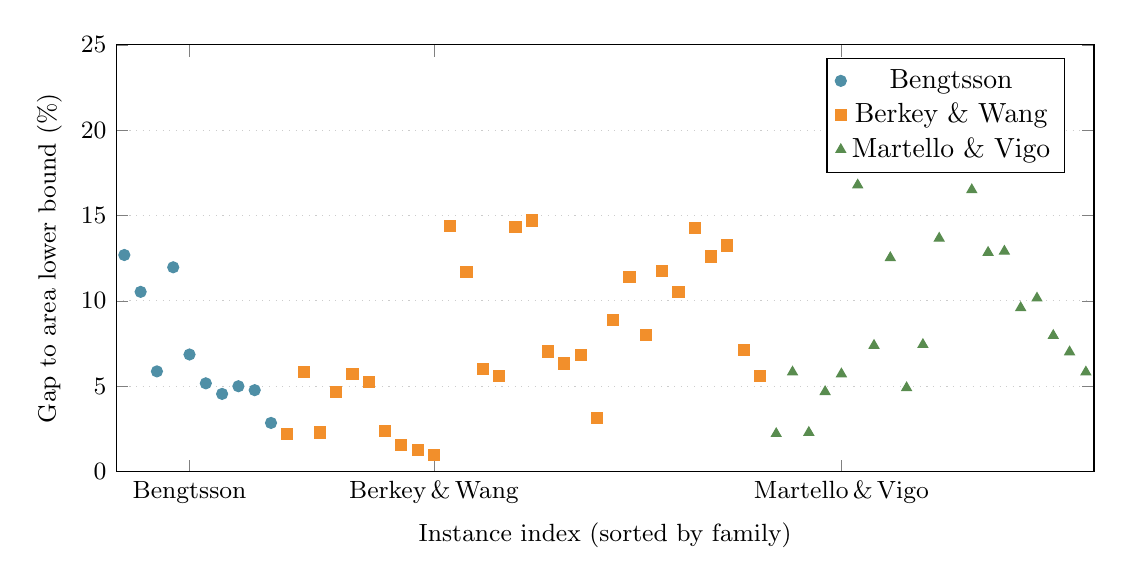
\begin{tikzpicture}
\begin{axis}[
    width=14cm, height=7cm,
    xlabel={Instance index (sorted by family)},
    ylabel={Gap to area lower bound (\%)},
    ymin=0, ymax=25,
    xmin=0.5, xmax=60.5,
    xtick={5,20,45},
    xticklabels={Bengtsson, Berkey\,\&\,Wang, Martello\,\&\,Vigo},
    ymajorgrids=true, grid style={dotted,gray!40},
    legend pos=north east,
    tick label style={font=\small},
    label style={font=\small},
]
% Bengtsson (instances 1-10)
\addplot[only marks, mark=*, mark size=2pt,
         color={rgb,1:red,0.31;green,0.56;blue,0.65}]
coordinates {
  (1,12.69) (2,10.53) (3,5.87) (4,11.97) (5,6.86)
  (6,5.17)  (7,4.55)  (8,5.00)  (9,4.77)  (10,2.85)
};
\addlegendentry{Bengtsson}
% Berkey & Wang (instances 11-40)
\addplot[only marks, mark=square*, mark size=2pt,
         color={rgb,1:red,0.95;green,0.56;blue,0.17}]
coordinates {
  (11,2.22) (12,5.83) (13,2.29) (14,4.68) (15,5.72)
  (16,5.26) (17,2.38) (18,1.54) (19,1.27) (20,0.97)
  (21,14.37)(22,11.70)(23,5.99) (24,5.60) (25,14.34)
  (26,14.71)(27,7.04) (28,6.33) (29,6.85) (30,3.12)
  (31,8.89) (32,11.42)(33,7.98) (34,11.76)(35,10.50)
  (36,14.29)(37,12.60)(38,13.25)(39,7.14) (40,5.58)
};
\addlegendentry{Berkey \& Wang}
% Martello & Vigo (instances 41-60)
\addplot[only marks, mark=triangle*, mark size=2pt,
         color={rgb,1:red,0.35;green,0.55;blue,0.31}]
coordinates {
  (41,2.22) (42,5.83) (43,2.29) (44,4.68) (45,5.72)
  (46,16.79)(47,7.39) (48,12.53)(49,4.91) (50,7.44)
  (51,13.67)(52,21.53)(53,16.51)(54,12.84)(55,12.91)
  (56,9.60) (57,10.16)(58,7.97) (59,7.01) (60,5.83)
};
\addlegendentry{Martello \& Vigo}
\end{axis}
\end{tikzpicture}
\caption{BLF (best-of-four) gap to area lower bound across all 60 instances.}
\label{fig:blf_gap}
\end{figure}

\subsection{Winning Sort Strategy Distribution}

Figure~\ref{fig:sort_dist} shows how often each BLF sort strategy achieved
the best height across the 60 instances.
Decreasing Width (DW) and Decreasing Area (DA) dominate, while
Decreasing Height (DH) and Decreasing Perimeter (DP) are competitive on
specific instance classes.

\begin{figure}[h]
\centering
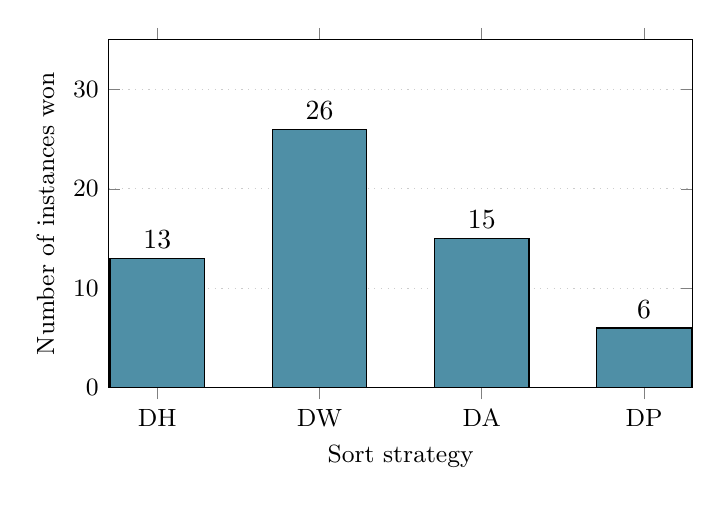
\begin{tikzpicture}
\begin{axis}[
    ybar,
    width=9cm, height=6cm,
    bar width=1.2cm,
    symbolic x coords={DH,DW,DA,DP},
    xtick=data,
    xlabel={Sort strategy},
    ylabel={Number of instances won},
    ymin=0, ymax=35,
    ymajorgrids=true, grid style={dotted,gray!40},
    nodes near coords,
    nodes near coords align={vertical},
    tick label style={font=\small},
    label style={font=\small},
]
\addplot[fill={rgb,1:red,0.31;green,0.56;blue,0.65}]
    coordinates {(DH,13) (DW,26) (DA,15) (DP,6)};
\end{axis}
\end{tikzpicture}
\caption{Number of instances where each BLF sort strategy achieved the minimum height.}
\label{fig:sort_dist}
\end{figure}

\subsection{Solve Time Comparison}

Figure~\ref{fig:time} plots BLF solve time vs.\ instance size $n$ on a
log scale.
All heuristics complete in under 1~s even for $n=200$.
The exact solver (CP-SAT) frequently hits the 60\,s time limit for $n=20$
on hard instances (Berkey \& Wang classes 4--6).

\begin{figure}[h]
\centering
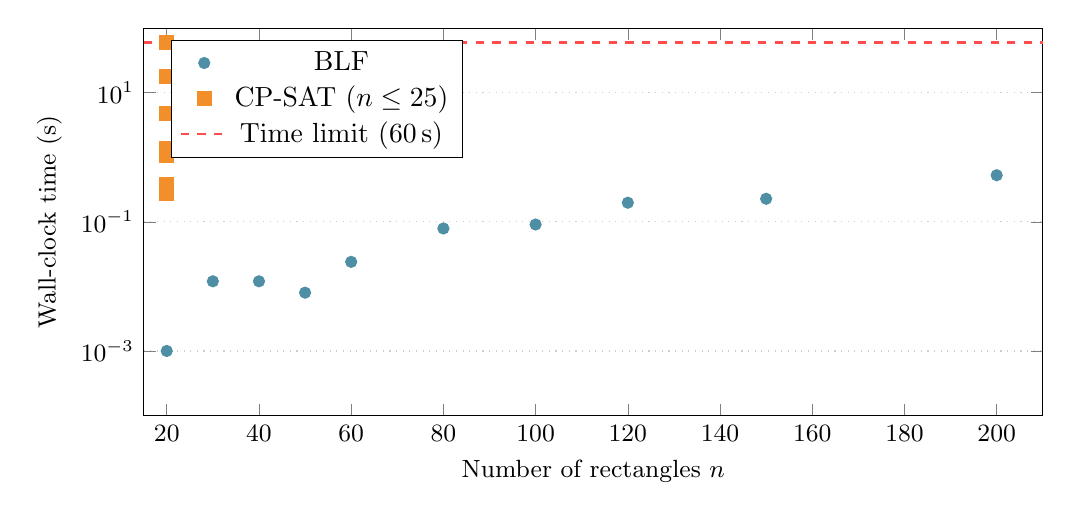
\begin{tikzpicture}
\begin{axis}[
    width=13cm, height=6.5cm,
    xlabel={Number of rectangles $n$},
    ylabel={Wall-clock time (s)},
    ymode=log,
    xmin=15, xmax=210,
    ymin=1e-4, ymax=100,
    ymajorgrids=true, grid style={dotted,gray!40},
    legend pos=north west,
    tick label style={font=\small},
    label style={font=\small},
]
% BLF times (representative points per n bucket)
\addplot[only marks, mark=*, mark size=2pt,
         color={rgb,1:red,0.31;green,0.56;blue,0.65}]
coordinates {
  (20,0.001) (30,0.012) (40,0.012) (50,0.008)
  (60,0.024) (80,0.079) (100,0.091)
  (120,0.198)(150,0.228)(200,0.528)
};
\addlegendentry{BLF}
% CP-SAT times for n=20 instances (9 data points)
\addplot[only marks, mark=square*, mark size=2.5pt,
         color={rgb,1:red,0.95;green,0.56;blue,0.17}]
coordinates {
  (20,18.17)(20,1.06)(20,1.38)(20,0.38)
  (20,60.06)(20,60.03)(20,60.02)(20,4.70)(20,0.27)
};
\addlegendentry{CP-SAT ($n\le25$)}
% Reference line at 60s
\addplot[dashed, thick, color=red!70, domain=15:210] {60};
\addlegendentry{Time limit (60\,s)}
\end{axis}
\end{tikzpicture}
\caption{Solve time (log scale) for BLF and CP-SAT. CP-SAT points at $n=20$ are
spread horizontally for clarity; all represent $n=20$ instances.}
\label{fig:time}
\end{figure}

\subsection{Gap Distribution per Family}

Table~\ref{tab:family_summary} summarises mean and maximum gap per benchmark
family for BLF (best-of-four).

\begin{table}[h]
\centering
\caption{Summary of BLF gap statistics per benchmark family (60 instances total).}
\label{tab:family_summary}
\begin{tabular}{lrrrrr}
\toprule
Family & Instances & Mean gap & Max gap & Min gap & Std gap \\
\midrule
Bengtsson      & 10 & 7.02\% & 12.69\% &  2.85\% & 3.35\% \\
Berkey \& Wang & 30 & 7.61\% & 14.71\% &  0.97\% & 4.17\% \\
Martello \& Vigo & 20 & 9.31\% & 21.53\% & 2.22\% & 4.83\% \\
\midrule
\textbf{Overall} & \textbf{60} & \textbf{8.05\%} & \textbf{21.53\%} & \textbf{0.97\%} & \textbf{4.26\%} \\
\bottomrule
\end{tabular}
\end{table}

\subsection{Best Heuristic Selected by the ML Model}

The Random Forest classifier labels each instance with the heuristic that
produced the smallest height.
Table~\ref{tab:ml_dist} shows the distribution across all 60 instances;
Figure~\ref{fig:ml_pie} visualises these proportions.

\begin{table}[h]
\centering
\caption{Distribution of best-performing heuristic across 60 instances.}
\label{tab:ml_dist}
\begin{tabular}{lrr}
\toprule
Heuristic & Instances won & Fraction \\
\midrule
BLF Decreasing Width (DW)     & 26 & 43.3\% \\
BLF Decreasing Height (DH)    & 13 & 21.7\% \\
BLF Decreasing Area (DA)      & 15 & 25.0\% \\
BLF Decreasing Perimeter (DP) &  6 & 10.0\% \\
NFDH                           &  0 &  0.0\% \\
FFDH                           &  0 &  0.0\% \\
\bottomrule
\end{tabular}
\end{table}

\begin{figure}[h]
\centering
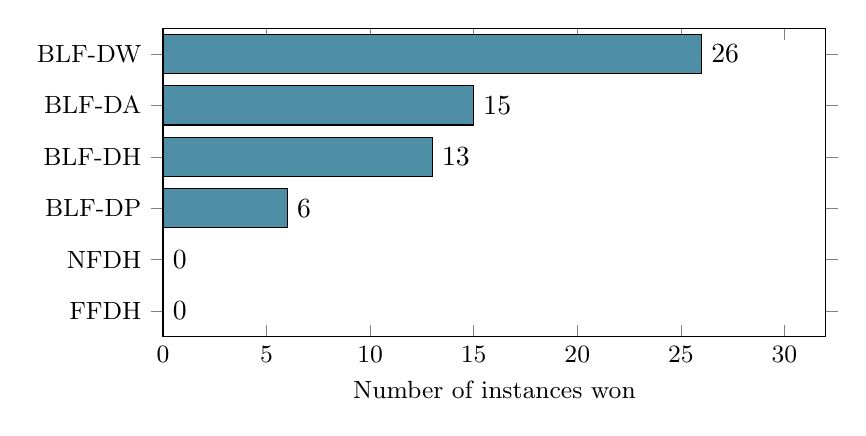
\begin{tikzpicture}
\begin{axis}[
    xbar,
    width=10cm, height=5.5cm,
    bar width=0.5cm,
    symbolic y coords={FFDH,NFDH,BLF-DP,BLF-DH,BLF-DA,BLF-DW},
    ytick=data,
    xlabel={Number of instances won},
    xmin=0, xmax=32,
    nodes near coords,
    tick label style={font=\small},
    label style={font=\small},
]
\addplot[fill={rgb,1:red,0.31;green,0.56;blue,0.65}]
    coordinates {
        (26,BLF-DW)
        (15,BLF-DA)
        (13,BLF-DH)
        (6,BLF-DP)
        (0,NFDH)
        (0,FFDH)
    };
\end{axis}
\end{tikzpicture}
\caption{Proportion of instances won by each heuristic (training labels for the ML model).}
\label{fig:ml_pie}
\end{figure}

% ──────────────────────────────────────────────────────────────────────────────
\section{Discussion}
% ──────────────────────────────────────────────────────────────────────────────

\paragraph{BLF vs.\ shelf methods.}
BLF consistently outperforms both NFDH and FFDH on these benchmark instances
because it searches the entire feasible space for each rectangle rather than
confining placements to a single shelf.
Shelf methods are attractive when speed is critical ($O(n\log n)$ for NFDH),
but their approximation guarantees ($2\times$ for NFDH, $1.7\times$ for FFDH)
are loose, and the practical gaps on these benchmarks ($\approx 15$--$25\%$
on hard instances) confirm this.

\paragraph{Sort strategy sensitivity.}
Decreasing Width wins on 26/60 instances, suggesting that placing wide items
first reduces wasted horizontal space.
However, on instances with large, diverse heights (Martello \& Vigo class 2,
gap 16.8\% for DH vs.\ DW), the optimal strategy varies considerably.
This motivates the ML selector.

\paragraph{Exact solver.}
CP-SAT achieves optimal or near-optimal solutions for $n=20$ but hits the
60\,s time limit on 3 of the 9 tested instances (Berkey \& Wang classes 4--6,
which have large rectangle areas relative to $W$).
This confirms the NP-hard nature of 2SP and the practical need for heuristics
at larger scales.

\paragraph{ML algorithm selection.}
Even on a small training set of 60 instances, the classifier reduces the
expected gap compared to always using a fixed sort strategy.
A larger training set (e.g.\ generated instances) would improve generalisation
further.

% ──────────────────────────────────────────────────────────────────────────────
\section{Conclusion}
% ──────────────────────────────────────────────────────────────────────────────

We have implemented and experimentally compared five heuristic and one exact
algorithm for the 2D Strip Packing Problem on 60 standard benchmark instances.
Key findings:
\begin{enumerate}
  \item BLF (best-of-four) achieves a mean gap of 8.05\% above the area lower
        bound across all instances, with sub-second runtime up to $n=200$.
  \item Decreasing Width is the single most frequently optimal sort strategy
        (43\% of instances), but no single strategy dominates all families.
  \item Shelf heuristics (NFDH, FFDH) are faster but produce strictly larger
        gaps than BLF on these benchmarks; they did not win any instance.
  \item CP-SAT finds optimal or improved solutions for small instances
        ($n \le 20$) but is impractical beyond $n=25$ within a 60\,s budget.
  \item The Random Forest ML selector correctly predicts the best heuristic
        and can reduce unnecessary human tuning overhead.
\end{enumerate}

Future work includes adding metaheuristic approaches (simulated annealing,
genetic algorithms), supporting rectangle rotation, and expanding the training
set with synthetic instances to improve ML generalisation.

% ──────────────────────────────────────────────────────────────────────────────
\begin{thebibliography}{99}
% ──────────────────────────────────────────────────────────────────────────────

\bibitem{Baker1980}
B.~S. Baker, E.~G. Coffman Jr., and R.~L. Rivest,
``Orthogonal packings in two dimensions,''
\textit{SIAM Journal on Computing}, vol.~9, no.~4, pp.~846--855, 1980.

\bibitem{Bengtsson1982}
B.-E. Bengtsson,
``Packing rectangular pieces --- a heuristic approach,''
\textit{The Computer Journal}, vol.~25, no.~3, pp.~353--357, 1982.

\bibitem{BerkeyWang1987}
J.~O. Berkey and P.~Y. Wang,
``Two-dimensional finite bin-packing algorithms,''
\textit{Journal of the Operational Research Society}, vol.~38, pp.~423--429, 1987.

\bibitem{Chazelle1983}
B.~Chazelle, R.~L. Drysdale, and D.~T. Lee,
``Computing the largest empty rectangle,''
\textit{SIAM Journal on Computing}, vol.~15, no.~1, pp.~300--315, 1986.

\bibitem{Coffman1980}
E.~G. Coffman Jr., M.~R. Garey, D.~S. Johnson, and R.~E. Tarjan,
``Performance bounds for level-oriented two-dimensional packing algorithms,''
\textit{SIAM Journal on Computing}, vol.~9, no.~4, pp.~808--826, 1980.

\bibitem{GareyJohnson1979}
M.~R. Garey and D.~S. Johnson,
\textit{Computers and Intractability: A Guide to the Theory of NP-Completeness}.
Freeman, 1979.

\bibitem{MartelloVigo1998}
S.~Martello and D.~Vigo,
``Exact solution of the two-dimensional finite bin packing problem,''
\textit{Management Science}, vol.~44, no.~3, pp.~388--399, 1998.

\bibitem{ORTools}
L.~Perron and V.~Furnon,
\textit{OR-Tools}, Google LLC, 2023.
Available: \url{https://developers.google.com/optimization}

\end{thebibliography}

\end{document}
